%!TEX program = xelatex
\documentclass[10pt,mathserif]{beamer}%,aspectratio=169 %画面比例16:9%
\usepackage{verbatimbox,color}
\usepackage{picinpar,graphicx}
\usepackage{smartdiagram}
\usesmartdiagramlibrary{additions}
\usepackage{multicol}
\usepackage{biblatex}
\usepackage{xmpmulti}
\usepackage{xeCJK}
\usepackage{hyperref} % links
\usepackage{pgfgantt}
\usepackage{pdfpages}
\usetheme[
 sidebar, xdblue
 ]{XDUstyle}
\usepackage{mdframed} 
\theoremstyle{definition}
\mdfdefinestyle{theoremstyle}{%
	linecolor=gray!40,linewidth=.5pt,%
	backgroundcolor=gray!10,
	skipabove=8pt,
	skipbelow=5pt,
	innerleftmargin=7pt,
	innerrightmargin=7pt,
	frametitlerule=true,%
	frametitlerulewidth=.5pt,
	frametitlebackgroundcolor=gray!15,
	frametitleaboveskip=0pt,
	frametitlebelowskip=0pt,
	innertopmargin=.4\baselineskip,
	innerbottommargin=.4\baselineskip,
	shadow=true,shadowsize=3pt,shadowcolor=black!20,
	theoremseparator={.},
}
%[section]means add the section number in the first place.
\mdtheorem[style=theoremstyle]{defi}{\hspace{0em}$\blacklozenge$定义}
\mdtheorem[style=theoremstyle]{solu}{\hspace{0em}$\checkmark$思路}

\title{高寒草地和温性草地植物多样性和微生物多样性关系沿水分梯度的对比研究}
%\subtitle{微生物生态学}
\institute[中国科学院大学\\生命科学学院]{指导老师:王艳芬} % 中括号部分为导航栏底所用尽可能精简
\author{张彪}
\date{2016年07月06日}% 时间可自行设置
	
\begin{document}%
{\xdbg \frame[plain,noframenumbering]{\titlepage}}%首页标题页

%\part{第一部分}
\AtBeginSection[]
{
	\begin{frame}[noframenumbering]{目录}
		\tableofcontents[subsectionstyle=hide]
	\end{frame}
	\begin{frame}[noframenumbering]{目录}
		\tableofcontents[currentsection,subsectionstyle=hide]
	\end{frame}
}
\section{选题背景及研究现状}

\subsection{选题背景}
\begin{frame}{\insertsection}{\insertsubsection}
	\begin{center}
		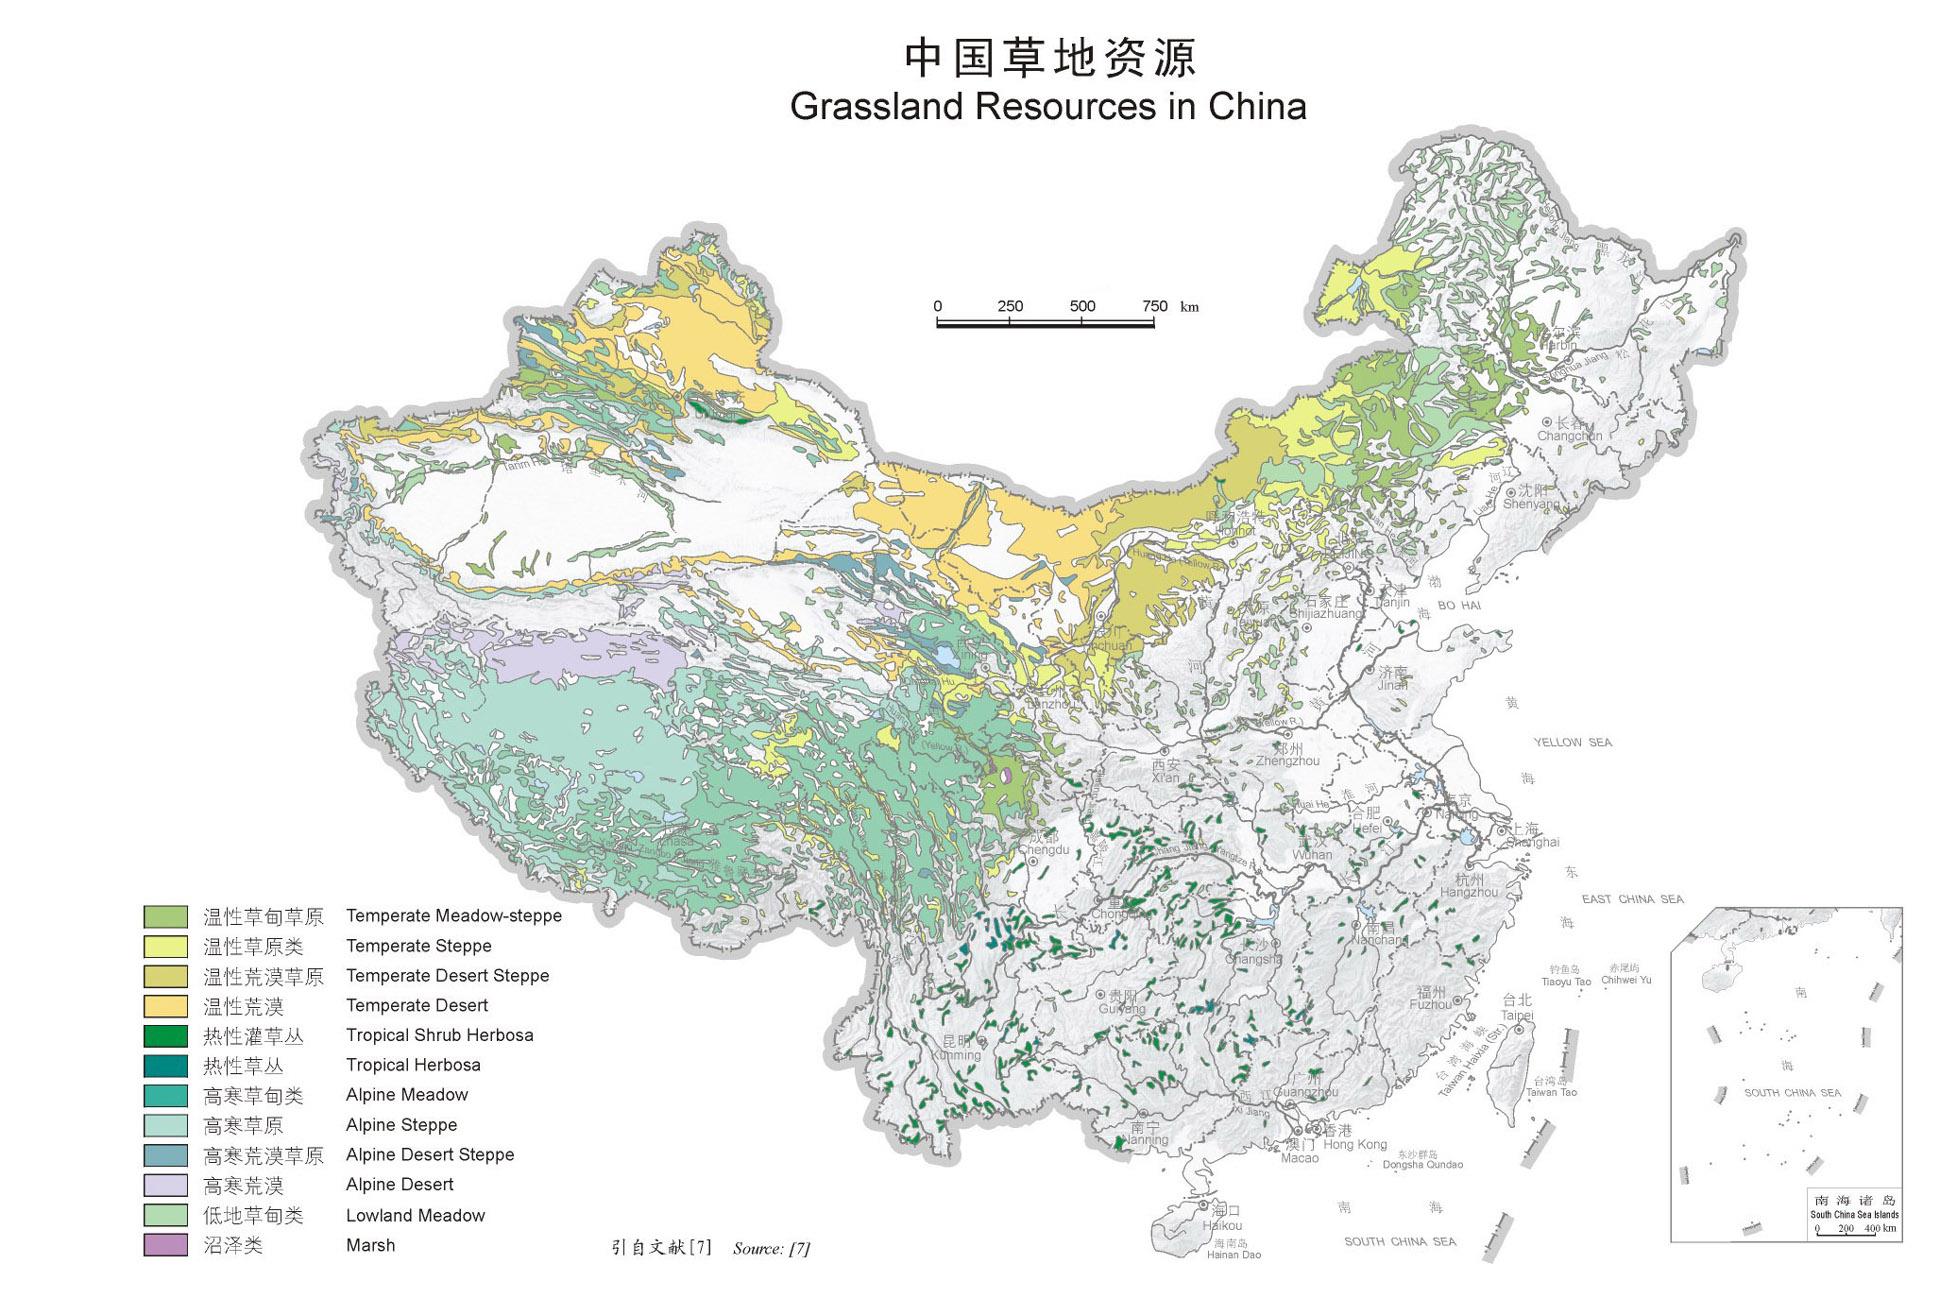
\includegraphics[width = 0.9\textwidth]{./pic/中国草地资源.jpg}
	\end{center}
\end{frame}
\begin{frame}{Fixing an Optical Mouse}
	\begin{columns}
		\column{0.7\textwidth}
		\hskip 15ex 中国草地资源
		\begin{center}
			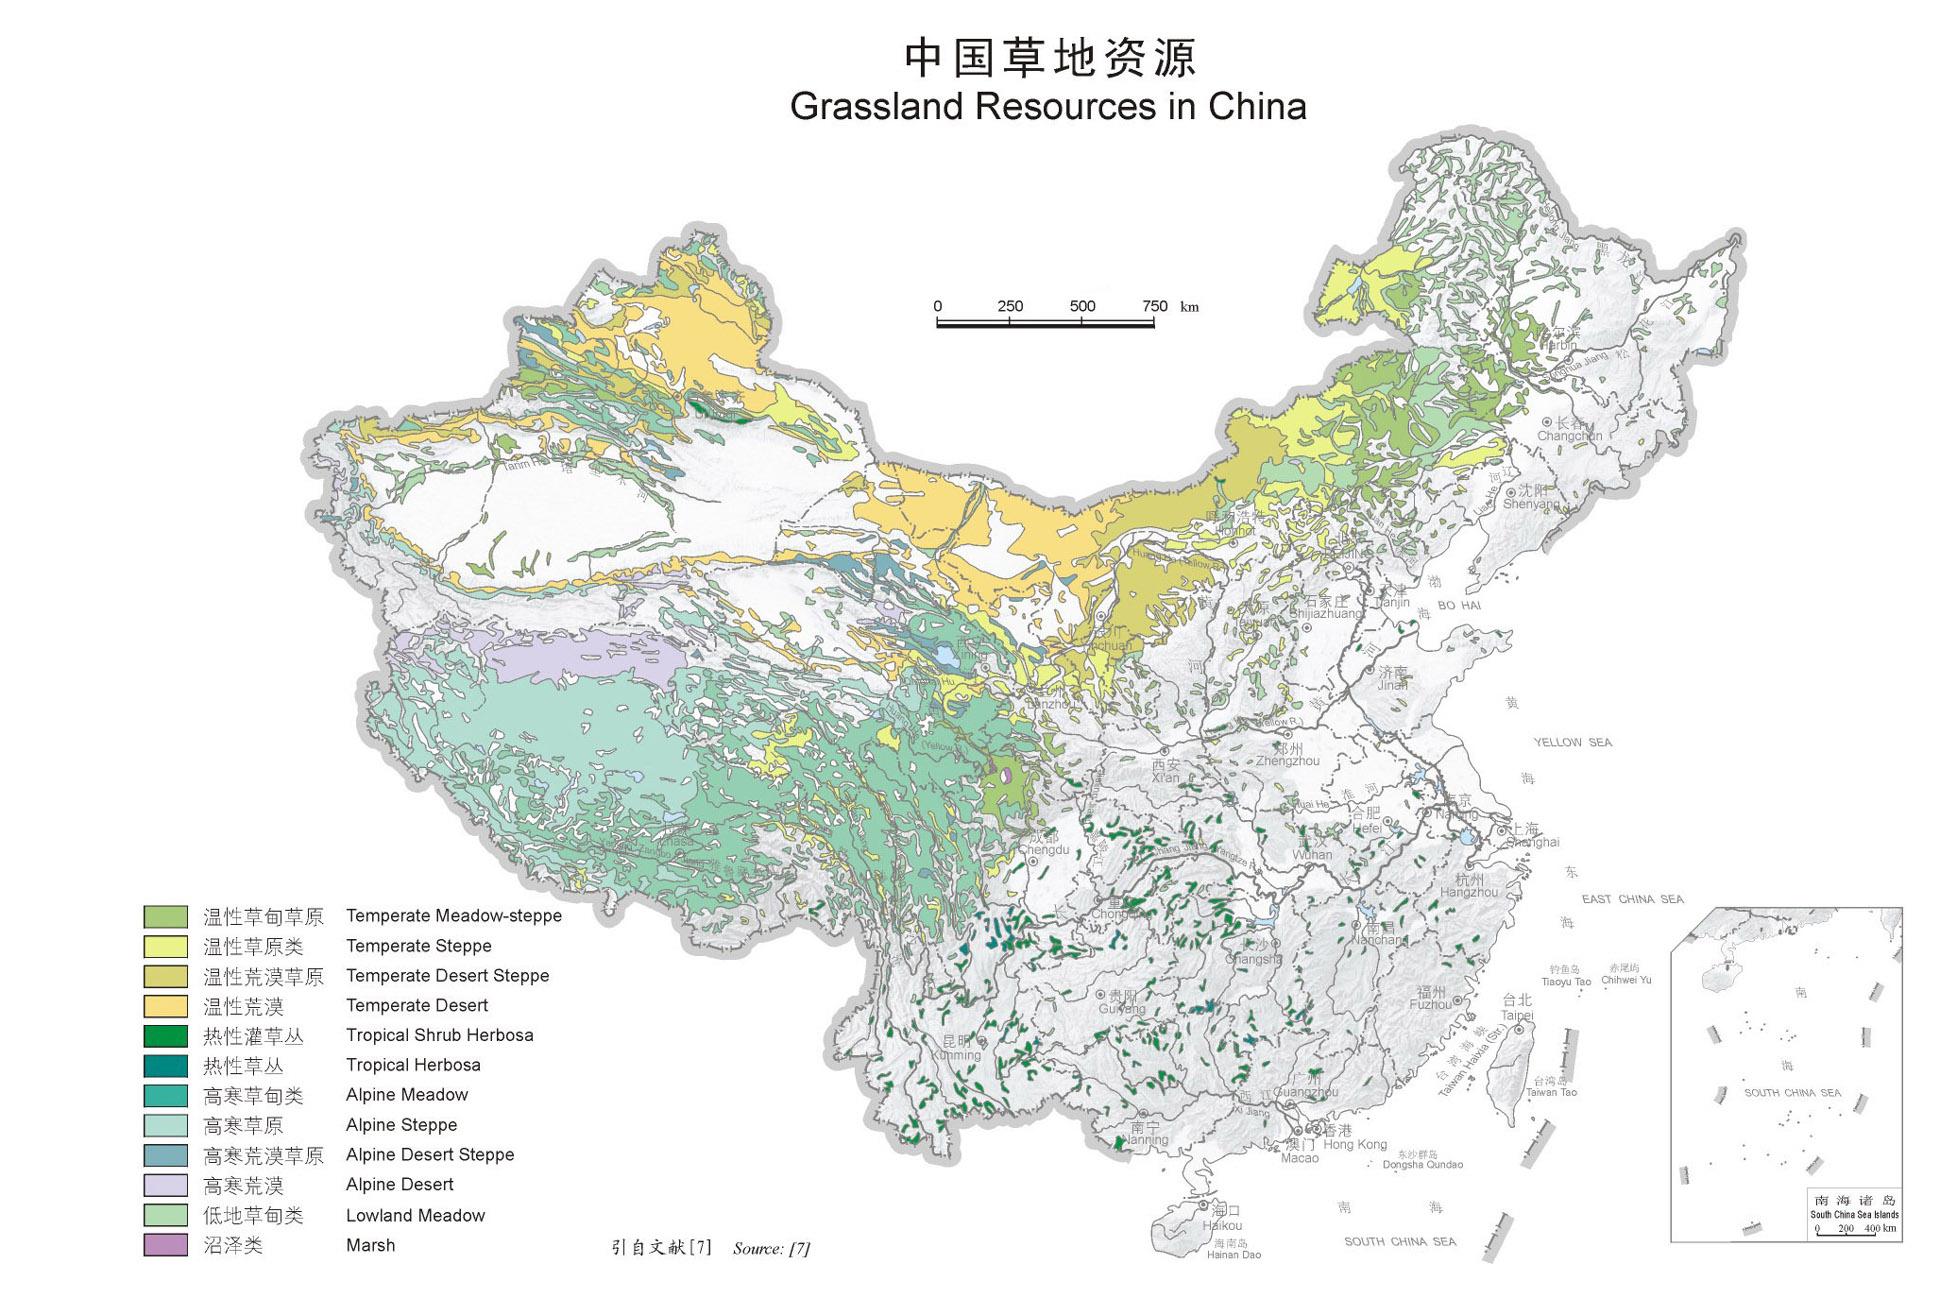
\includegraphics[width = 0.9\textwidth]{./pic/中国草地资源.jpg}
		\end{center}
		%\vspace{15mm}
		\only<6>{
		我国是世界上第二大草地资源大国,天然草原面积3.94×108hm2,约占我国国土面积的41.7\%,是耕地面积的3 倍左右,林地面积的2 倍多(刘黎明,2002)。
	    }
		\column{0.3\textwidth}
		主要分布					
		\begin{itemize}
			\item<1-> 东北平原
			\item<2-> 内蒙古高原
			\item<3-> 黄土高原
			\item<4-> 青藏高原
			\item<5-> 新疆山地
		\end{itemize}
	\end{columns}
\end{frame}

\subsection{研究现状}
\begin{frame}{\insertsection}{\insertsubsection}
	\begin{center}
		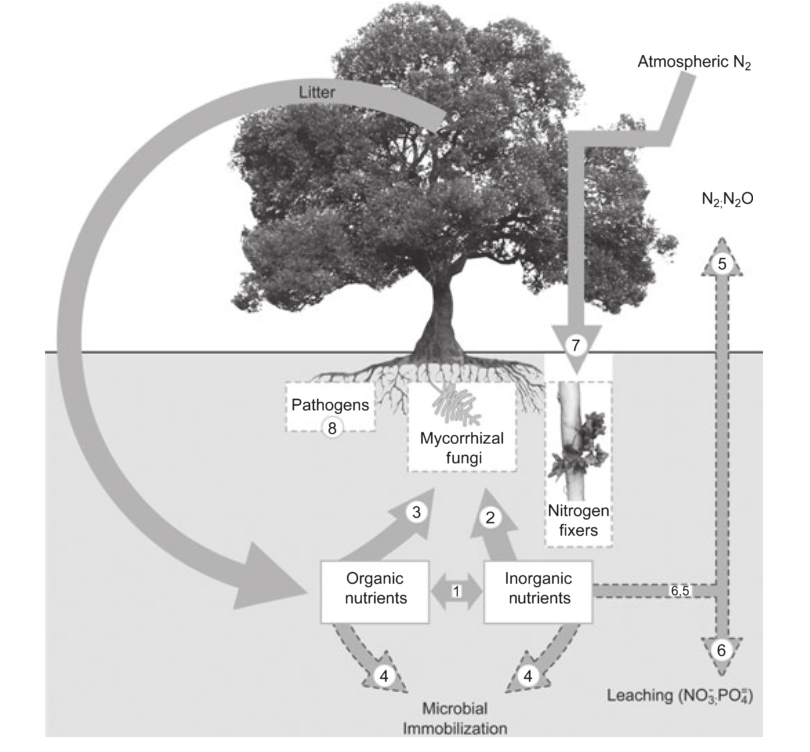
\includegraphics[width = 0.9\textwidth]{./pic/微生物养分和植物互相影响.jpg}
	\end{center}
\end{frame}
\begin{frame}{\insertsection}{\insertsubsection}
	\begin{columns}
		\column{0.5\textwidth}
		植物物种多样性与微生物多样性的关系	
		\begin{center}
			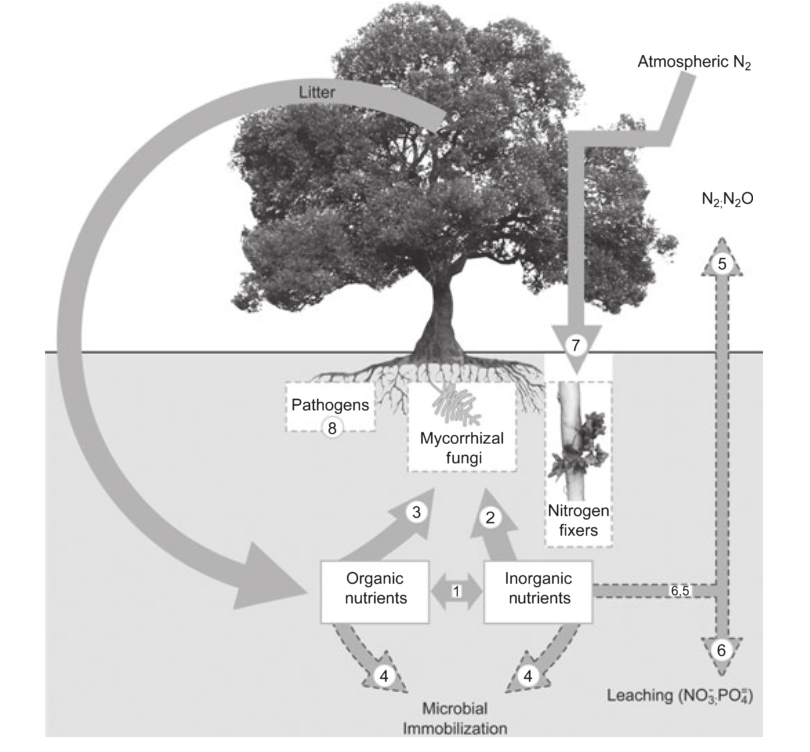
\includegraphics[width = 0.9\textwidth]{./pic/微生物养分和植物互相影响.jpg}
		\end{center}
		
		\column{0.5\textwidth}
		植物多样性通过几个方面对微生物产生直接或间接影响:
		\begin{itemize}
			\item<1-> 提高净初级生产力(NPP)
			\item<2-> 提高凋落物的多样性
			\item<3-> 提高食物资源和生境的多样性
			\item<4-> 改变凋落物的质量(C/N)
			\item<5-> 根分泌物的多样性
			\item<6-> 土壤温度、湿度、pH
		\end{itemize}
	\end{columns}
\end{frame}
\begin{frame}{\insertsection}{\insertsubsection}
	\begin{center}
		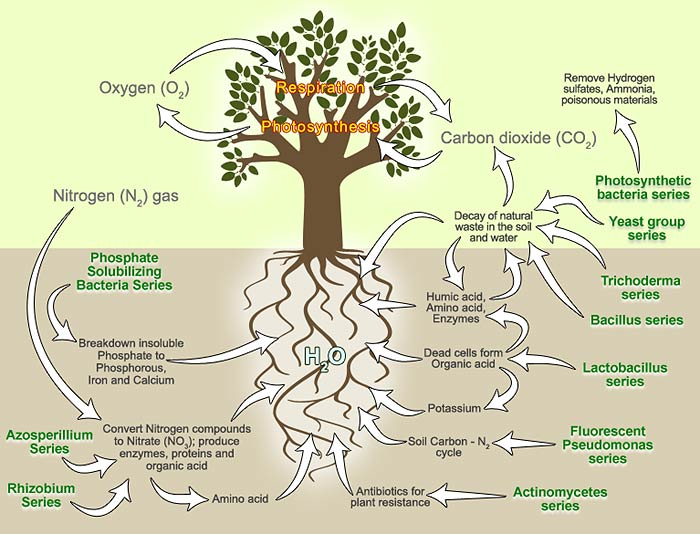
\includegraphics[width = 0.9\textwidth]{./pic/地下微生物群落.jpg}
	\end{center}
\end{frame}
\begin{frame}{\insertsection}{\insertsubsection}
	\begin{columns}
		\column{0.5\textwidth}
		地下微生物群落	
		\begin{center}
			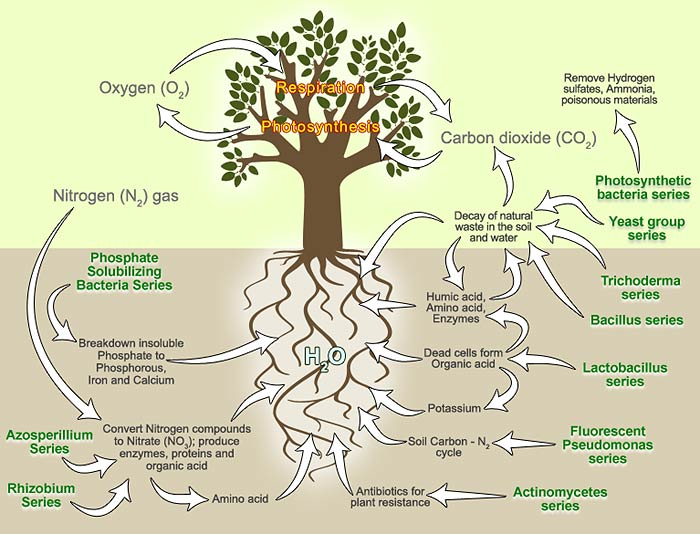
\includegraphics[width = 0.9\textwidth]{./pic/地下微生物群落.jpg}
		\end{center}
		
		\column{0.5\textwidth}
		地下微生物群落在决定植物群落生产力、多样性和组成中发挥着重要作用(Kulmatiski et al., 2011)。前人的研究结果表明,地下微生物多样性会影响植物生长和生产力、有效养分、生态系统功能。还有一些研究显示微生物群落组成的变化会反馈植物的协同生存(Reynolds et al., 2003)和群落组成(Bever, 2003)。
	\end{columns}
\end{frame}




\subsection{研究现状}
\begin{frame}{\insertsection}{\insertsubsection}
\begin{center}
	\usetikzlibrary{shapes.geometric} % required in the preamble
	\smartdiagramset{
		uniform color list=gray!60!black for 6 items,
		font=\large,
		module minimum width=2.5cm,
		module minimum height=1.5cm,
		text width=1cm,
		circular distance=3cm,
		circular final arrow disabled=true,
	}
	\smartdiagram[circular diagram:clockwise]{植物多样性,冠层密度,土表蒸发,土壤水分,微生物多样性}
\end{center}
\end{frame}
\begin{frame}{\insertsection}{\insertsubsection}
	
\end{frame}
\begin{frame}{\insertsection}{\insertsubsection}
	
\end{frame}
\begin{frame}{\insertsection}{\insertsubsection}
	
\end{frame}


\subsection{研究目的}
\begin{frame}{\insertsection}{\insertsubsection}
	\begin{itemize}
		\item 沿水分梯度条件下,高寒草地和温性草地植物物种多样性和微生物多样性的关系
		\item 沿水分梯度条件下,高寒草地和温性草地植物功能群多样性与微生物多样性的关系
		\item 在不同生态系统类型条件下,植物物种多样性和功能群多样性对微生物多样性的影响
	\end{itemize}
\end{frame}
\section{研究方法、技术路线、实验方案}
\subsection{研究方法}
\begin{frame}{\insertsubsection——常见方法}
	\begin{columns}
		\column{0.35\textwidth}
		常见的研究方法:
		\begin{itemize}
			\item<1-> 植物多样性梯度
			\item<2-> 土壤微生物多样性梯度
			\item<3-> 演替梯度
			\item<4-> 环境因子梯度
			\item<5-> 功能群移除			
		\end{itemize}
		\column{0.65\textwidth}
		\begin{center}
			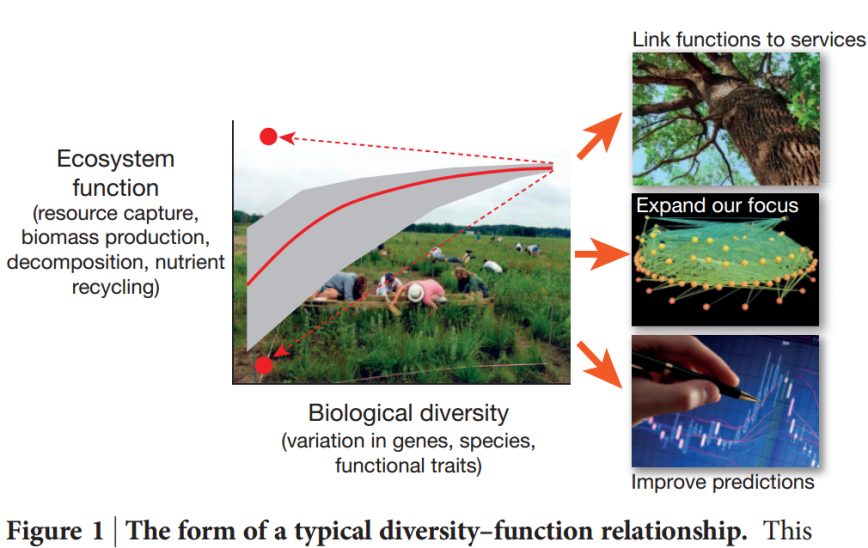
\includegraphics[width = \textwidth]{./pic/2.1.1.png}
		\end{center}
	\end{columns}
\end{frame}
\begin{frame}{\insertsubsection——研究地点}
	\begin{center}
		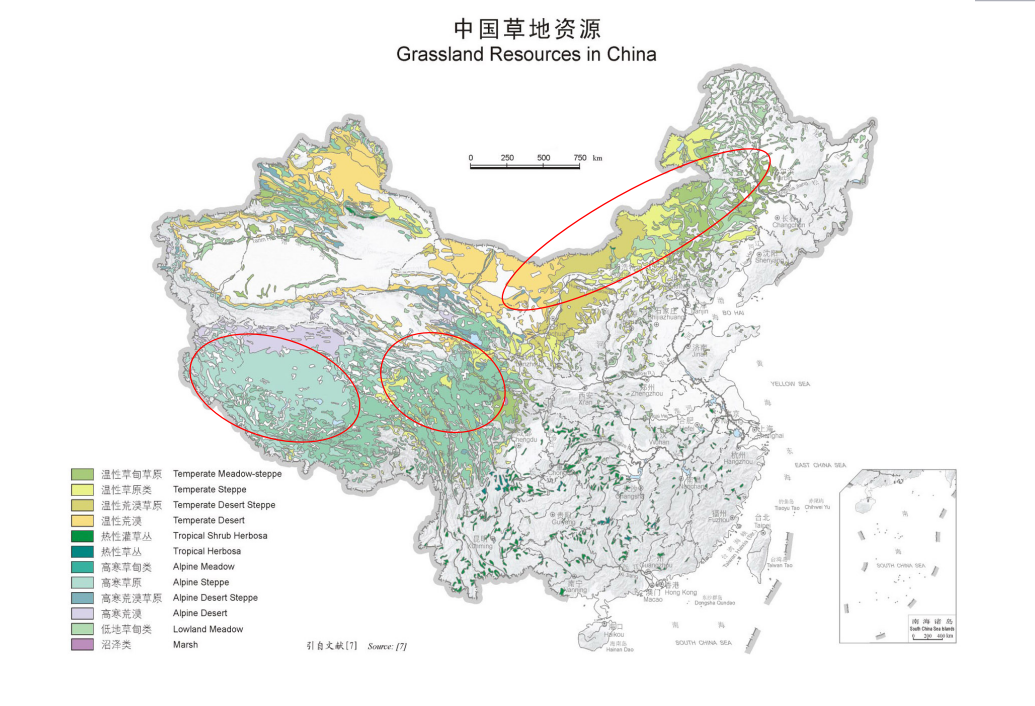
\includegraphics[width = 0.9\textwidth]{./pic/2.1.2.png}
	\end{center}
	研究地点:
	
	西藏、青海、内蒙古南北两条平行样带
\end{frame}
\begin{frame}{\insertsubsection——土壤理化性质参数}	
	
	把样带采集的土壤过筛(1mm×1mm)除去根,置于背光条件下自然风干备用。
	\vskip 2em
	1)TOC;2)TN;
	3)TP;4)MBC;
	5)MBN;\\
	6)NH4-N;7)NO3-N;8)有效P;
	9)pH
\end{frame}
\begin{frame}{\insertsubsection——植物多样性参数}
	
	$\alpha$多样性:丰富度指数(Richness), Shannon-Winer多样性指数($H'$)
	\begin{equation}\label{f_1}
	H'=-\sum_{i=1}^{S}P_i lnP_i
	\end{equation}	
	式(\ref{f_1})中$S$为物种数,$P_i$为第$i$种个体所占总个体数的比例。
\end{frame}
\begin{frame}{\insertsubsection——植物多样性参数}	
	$\beta$多样性:Bray-Curtis指数:
	\begin{equation}\label{f_2}
	 CI=\frac{2jI}{aI+bI}
	\end{equation}	
	式(\ref{f_2})中,$jI$为样地$A(jI a)$和样地$B(jI b)$共有种物种重要值较小者之和;	
	\begin{equation}\label{f_3}
	jI=\sum min(jIa+jIb)
	\end{equation}
\end{frame}
\begin{frame}{\insertsubsection——室内试验}
	
	
		\begin{center}
			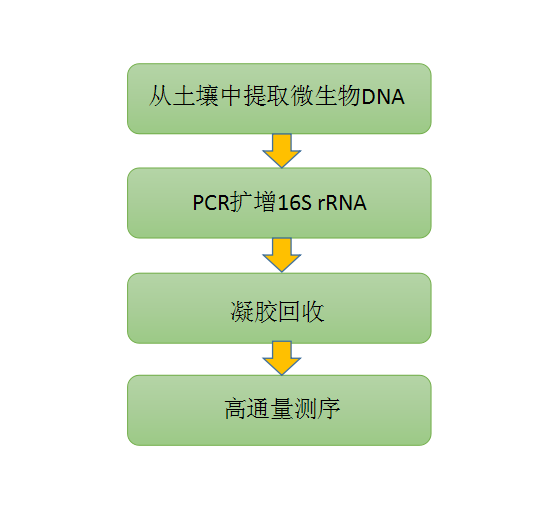
\includegraphics[width = 0.6\textwidth]{./pic/2.1.3.png}
		\end{center}
\end{frame}


\subsection{技术路线}
\begin{frame}{\insertsubsection}
	\begin{center}
		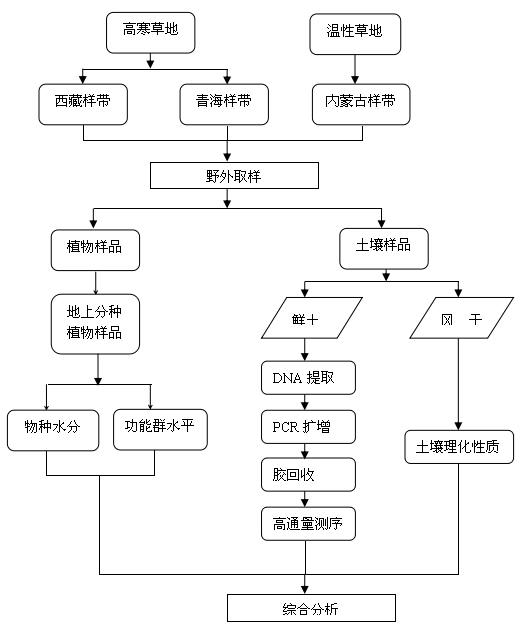
\includegraphics[width = 0.6\textwidth]{./pic/技术路线.jpg}
	\end{center}
\end{frame}
\subsection{实验方案}
\begin{frame}{\insertsubsection}
	\begin{center}
		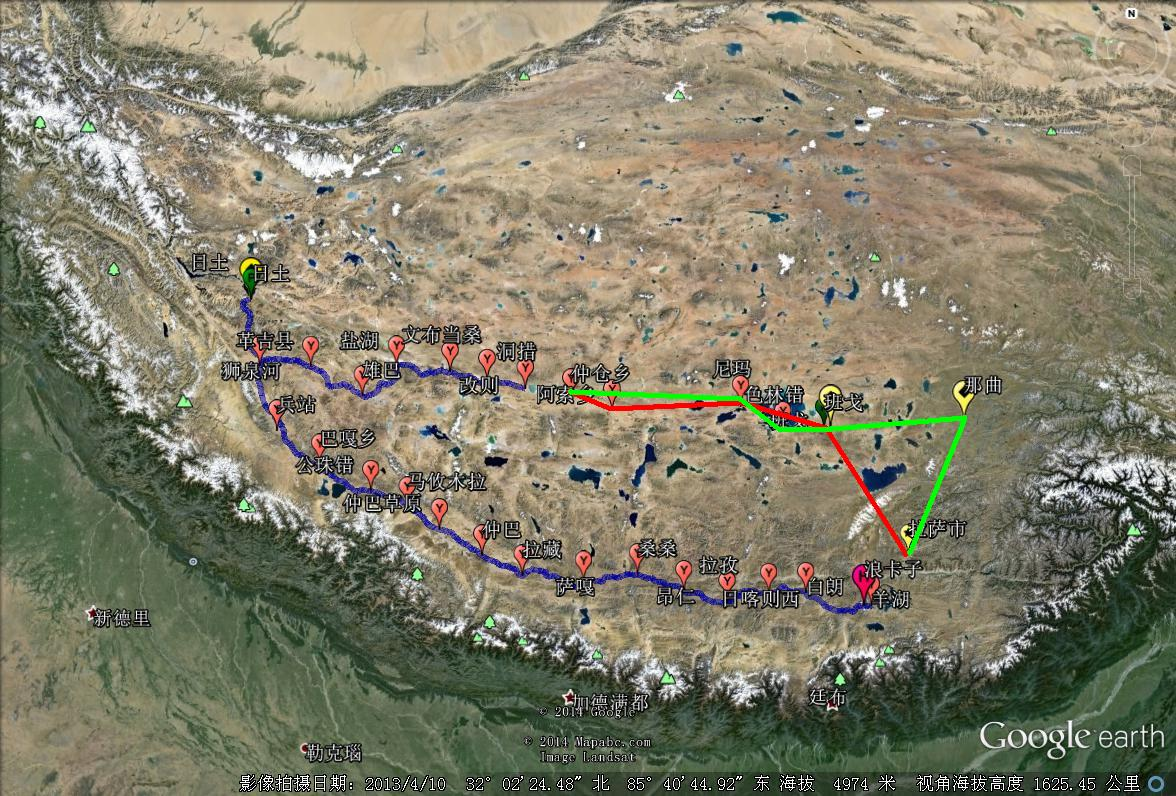
\includegraphics[width = 0.9\textwidth]{./pic/西藏瓦岗.jpg}
	\end{center}
	1)在西藏冈底斯山脉南北两侧,沿水分梯度各由东往西定点取样;
\end{frame}

\begin{frame}{\insertsubsection}	
	\begin{columns}
		\column{0.5\textwidth}
		\begin{center}
			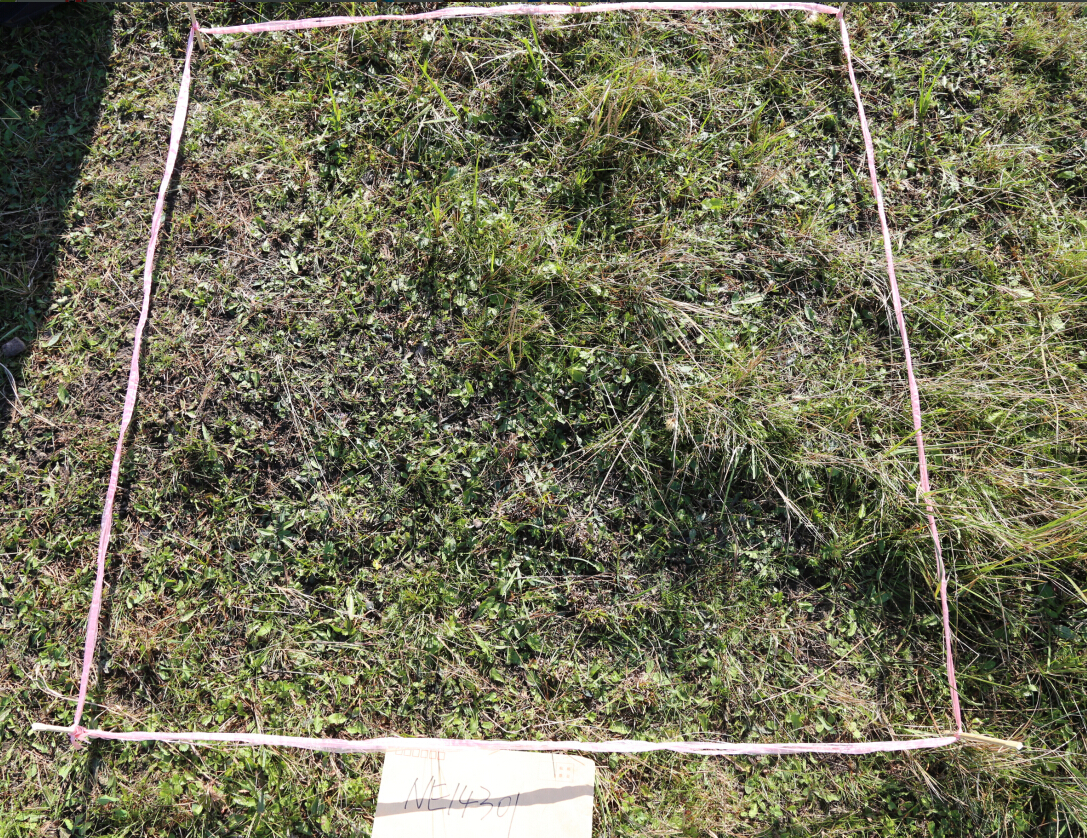
\includegraphics[width = 1.1\textwidth]{./pic/2.3.1.jpg}
		\end{center}		
		\column{0.5\textwidth}
		\begin{center}
			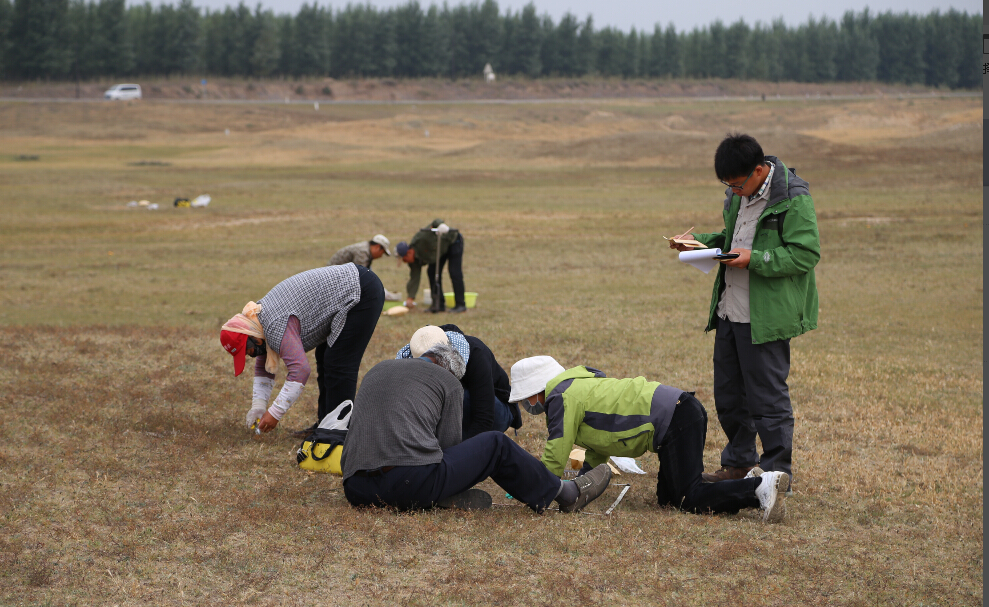
\includegraphics[width = 1.4\textwidth]{./pic/2.3.2.jpg}
		\end{center}
	\end{columns}
	\vskip 2em
	2)在每个取样点,随机选择5个1m×1m的样方,记录每个物种(随机选取5株)的高度,分种剪取地上植物生物量,称鲜重,实验室65℃烘72小时,称干重;	
\end{frame}
\begin{frame}{\insertsubsection}	
	\begin{columns}
		\column{0.5\textwidth}
		\begin{center}
			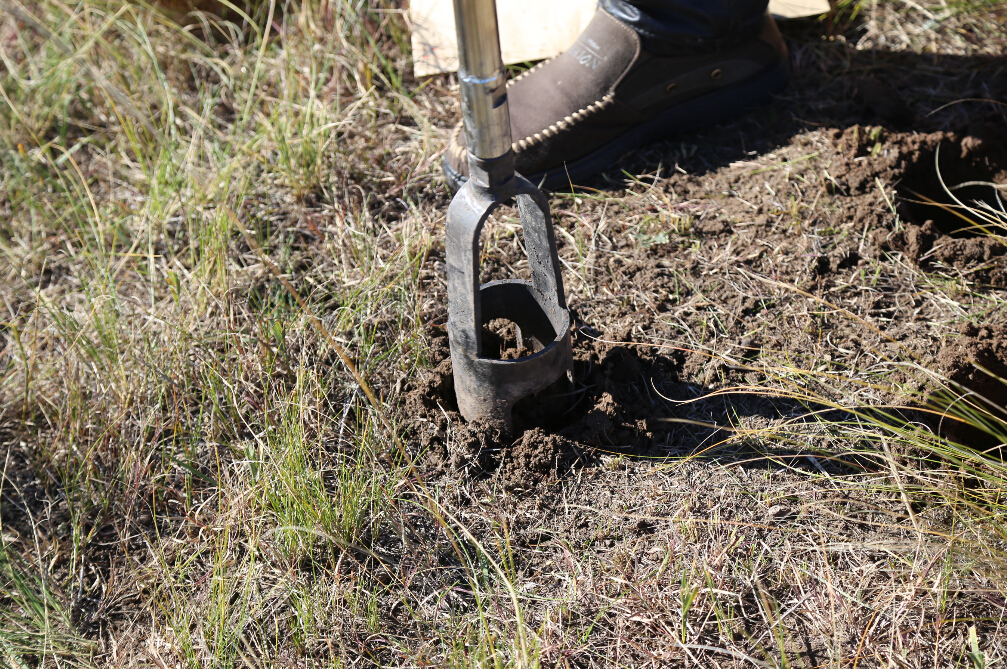
\includegraphics[width = 1.1\textwidth]{./pic/2.3.3.jpg}
		\end{center}		
		\column{0.5\textwidth}	
		\begin{center}
			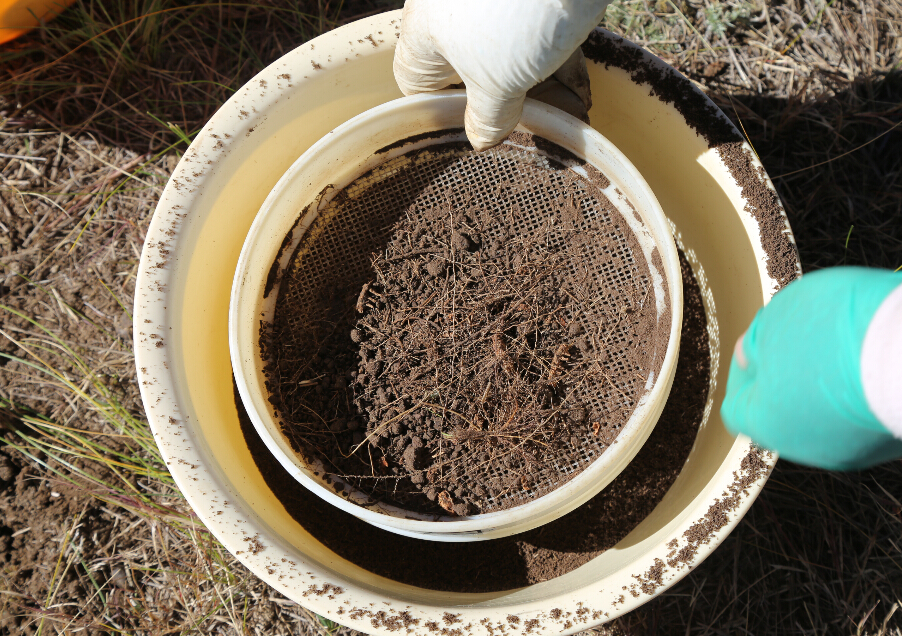
\includegraphics[width = 1.05\textwidth]{./pic/2.3.4.jpg}
		\end{center}
	\end{columns}
	\vskip 2em
	3)在每个取样点随即选择的5个1m×1m的样方剪除地上生物量后,用5cm根钻每层(0-10cm、10-20cm、20-30cm)取3钻土壤样品并均匀混合,一半土壤样品迅速放入野外冰箱并冷冻保存,用于提取微生物DNA;另外一半带回实验室风干,用于测量土壤的理化性质;	
\end{frame}

\begin{frame}{\insertsubsection}
\begin{center}
	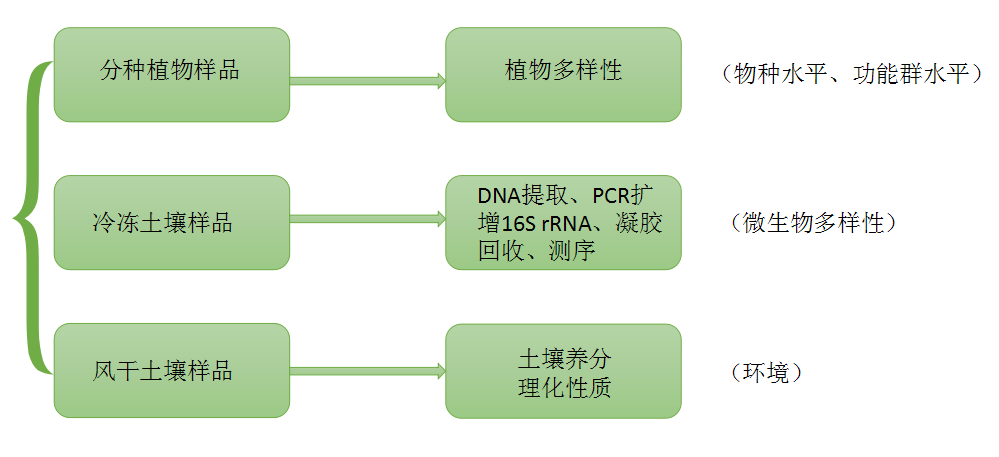
\includegraphics[width =\textwidth]{./pic/2.3.5.png}
\end{center}
\end{frame}



\section{现阶段研究基础}
\begin{frame}{\insertsection——野外取样}
	\begin{center}
		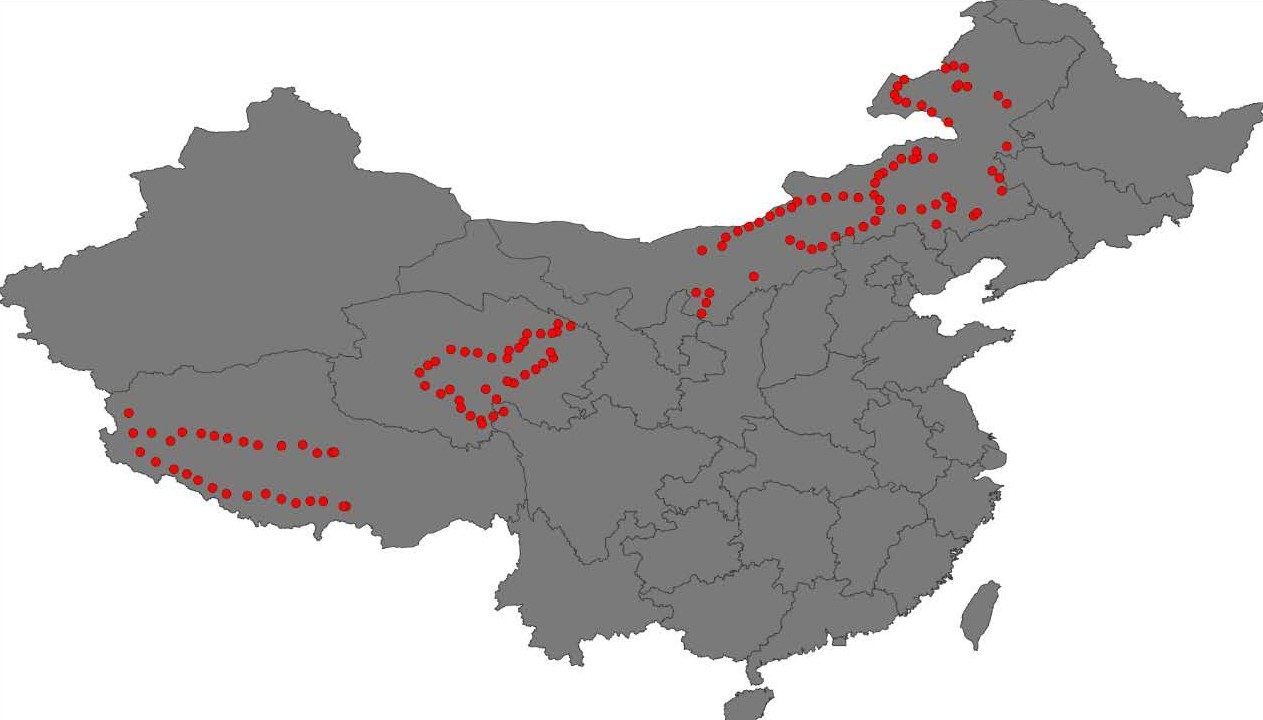
\includegraphics[width = 0.9\textwidth]{./pic/3.1.jpg}
	\end{center}
	126个样点
	\begin{itemize}
		\item 2014-8	西藏:28个样点, 青海:33个样点
		\item 2015-9	内蒙古:65样点
	\end{itemize}
\end{frame}

\subsection{植物样品}
\begin{frame}{\insertsection——植物样品}
		\begin{center}
			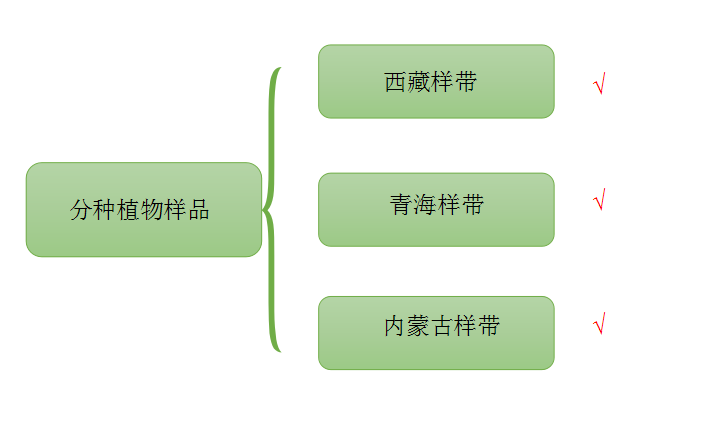
\includegraphics[width = \textwidth]{./pic/3.2.png}
		\end{center}
\end{frame}
\subsection{冷冻土壤样品}
\begin{frame}{\insertsection——冷冻土壤样品}
	\begin{center}
		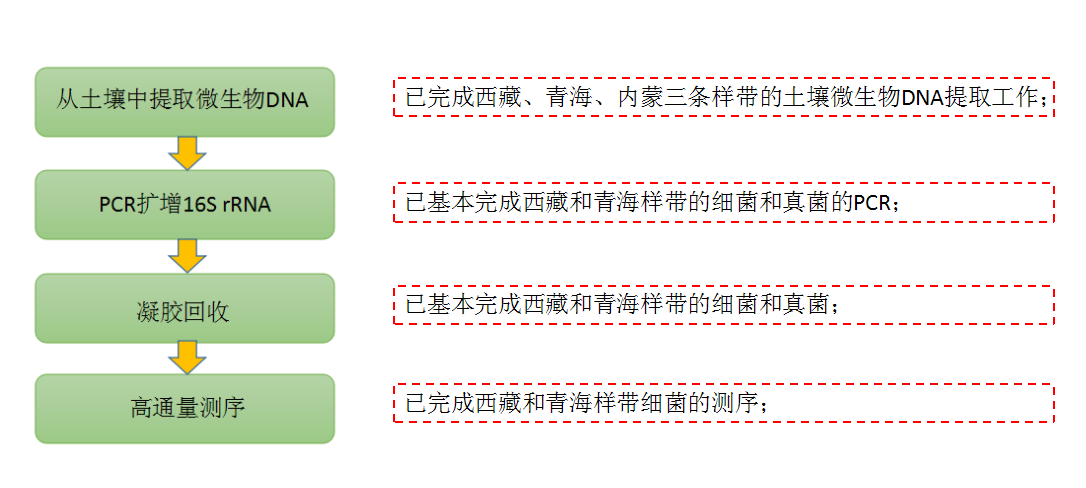
\includegraphics[width = \textwidth]{./pic/3.3.png}
	\end{center}
\end{frame}
\subsection{风干土壤样品}
\begin{frame}{\insertsection——风干土壤样品}
		\begin{center}
			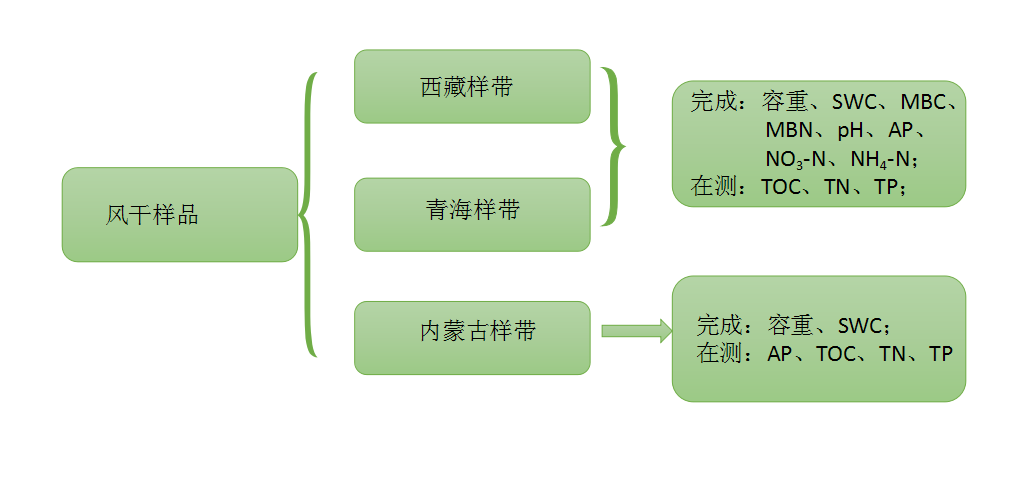
\includegraphics[width = \textwidth]{./pic/3.4.png}
		\end{center}
\end{frame}

\section{研究计划与工作安排}
\begin{frame}{\insertsection}{\insertsubsection}
\begin{center}
	\begin{tabular}{ l l  }
		2016.07-2016.10: & 对以往研究进行Meta分析;\\ 
		2016.10-2016.10: & 野外补样;\\
		2016.11-2017.01: & 分析青海样带植物多样性与\\
		& 微生物多样性的关系;\\
		2017.02-2017.06: & 分析西藏样带植多样性与\\
		& 微生物多样性的关系并撰写文章;\\  
		2017.12-2017.12: & 中期答辩\\
		2018.01-2018.03: & 博士学位论文撰写\\
		2018.05-2018.05: & 毕业答辩
	\end{tabular}
\end{center}

\end{frame}
\begin{frame}{\insertsection}{\insertsubsection}
	\begin{center}
		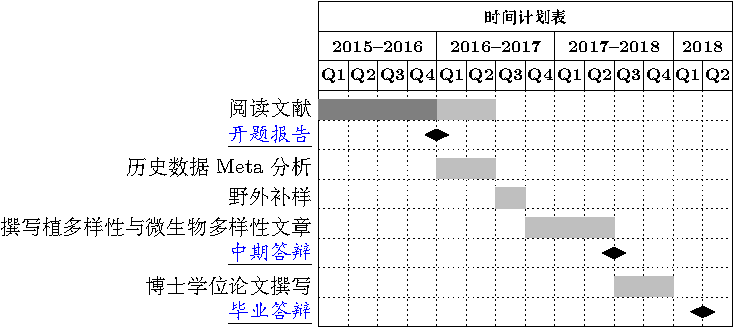
\includegraphics[width = \textwidth]{./pic/gatt.pdf}
	\end{center}
\end{frame}




{\xdbg%末页致谢
\begin{frame}[plain,noframenumbering]
 \finalpage{{\huge 感谢观看!}}
\end{frame}}


\end{document} 
